%% 
%% Copyright 2007, 2008, 2009 Elsevier Ltd
%% 
%% This file is part of the 'Elsarticle Bundle'.
%% ---------------------------------------------
%% 
%% It may be distributed under the conditions of the LaTeX Project Public
%% License, either version 1.2 of this license or (at your option) any
%% later version.  The latest version of this license is in
%%    http://www.latex-project.org/lppl.txt
%% and version 1.2 or later is part of all distributions of LaTeX
%% version 1999/12/01 or later.
%% 
%% The list of all files belonging to the 'Elsarticle Bundle' is
%% given in the file `manifest.txt'.
%% 

%% Template article for Elsevier's document class `elsarticle'
%% with numbered style bibliographic references
%% SP 2008/03/01

\documentclass[preprint,12pt]{elsarticle}

%% Use the option review to obtain double line spacing
%% \documentclass[authoryear,preprint,review,12pt]{elsarticle}

%% Use the options 1p,twocolumn; 3p; 3p,twocolumn; 5p; or 5p,twocolumn
%% for a journal layout:
%% \documentclass[final,1p,times]{elsarticle}
%% \documentclass[final,1p,times,twocolumn]{elsarticle}
%% \documentclass[final,3p,times]{elsarticle}
%% \documentclass[final,3p,times,twocolumn]{elsarticle}
%% \documentclass[final,5p,times]{elsarticle}
%% \documentclass[final,5p,times,twocolumn]{elsarticle}

%% For including figures, graphicx.sty has been loaded in
%% elsarticle.cls. If you prefer to use the old commands
%% please give \usepackage{epsfig}

%% The amssymb package provides various useful mathematical symbols
\usepackage{amssymb}

\usepackage{xeCJK}
\usepackage{subfig}

%% The amsthm package provides extended theorem environments
%% \usepackage{amsthm}

%% The lineno packages adds line numbers. Start line numbering with
%% \begin{linenumbers}, end it with \end{linenumbers}. Or switch it on
%% for the whole article with \linenumbers.
%% \usepackage{lineno}

\journal{CSP2016-期末论文}

\begin{document}

\begin{frontmatter}

%% Title, authors and addresses

%% use the tnoteref command within \title for footnotes;
%% use the tnotetext command for theassociated footnote;
%% use the fnref command within \author or \address for footnotes;
%% use the fntext command for theassociated footnote;
%% use the corref command within \author for corresponding author footnotes;
%% use the cortext command for theassociated footnote;
%% use the ead command for the email address,
%% and the form \ead[url] for the home page:
%% \title{Title\tnoteref{label1}}
%% \tnotetext[label1]{}
%% \author{Name\corref{cor1}\fnref{label2}}
%% \ead{email address}
%% \ead[url]{home page}
%% \fntext[label2]{}
%% \cortext[cor1]{}
%% \address{Address\fnref{label3}}
%% \fntext[label3]{}

\title{Sandboxing相关技术研究与思考}

%% use optional labels to link authors explicitly to addresses:
%% \author[label1,label2]{}
%% \address[label1]{}
%% \address[label2]{}

\author{尹至达}
\author{高策}

\address{上海交通大学软件学院}

\begin{abstract}

目前,互联网上的攻击越来越频繁,攻击者会通过各种攻击方式,以达到获取系统高权限,读取敏感数据等等攻击目的。沙箱作为一个用来隔离程序执行环境,使得程序在一个低权限的,高度隔离的环境中执行的技术,受到了越来越多的关注。本文以一个现代的浏览器为出发点,介绍了两类沙箱技术在其中的应用与体现,进而总结对比各种沙箱实现的特点,并且在最后对沙箱技术下一步的研究方向提出了看法。

\end{abstract}

\begin{keyword}
%% keywords here, in the form: keyword \sep keyword

%% PACS codes here, in the form: \PACS code \sep code

%% MSC codes here, in the form: \MSC code \sep code
%% or \MSC[2008] code \sep code (2000 is the default)

Sandboxing \sep System Call Interposition \sep Capabilities \sep Software-based Fault Isolation

\end{keyword}

\end{frontmatter}

%% \linenumbers

%% main text
\section{引言}
\label{s:introduction}

随着网络全球化的发展,安全越来越成为了一个进入大众视野的议题。互联网在提供给用户以便利的同时,也对隐私安全提出了新的挑战。这样的问题存在于各种平台上,攻击者会将诸如木马、病毒、恶意软件等等内容发布到被攻击者的终端上。\cite{miwa} 虽然现在的操作系统上的安全措施已经足够强大到防止绝大多数的攻击,但是用户总是期望更加安全的环境。而沙箱是一种非常实用的安全机制,通过引入沙箱技术,程序可以在隔离的环境中运行,使得程序的运行不会影响操作系统,同时操作系统也不会影响到程序。在传统的操作系统的抽象中,用户的应用对于系统各种资源的使用都是无限制的,而沙箱技术是对其运行时环境的隔离 \cite{sandbox}。

\begin{figure*}
\centering
\subfloat[第一类沙箱]{
\label{fig:t1sb}
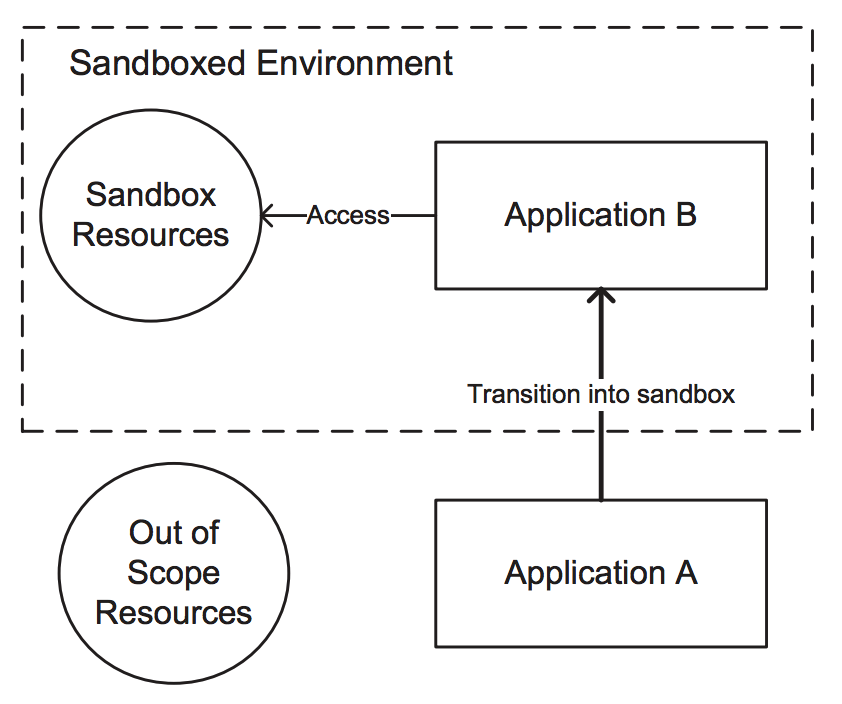
\includegraphics[width=0.4\linewidth]{imgs/type-1-sandbox.png}
}
\subfloat[第二类沙箱]{
\label{fig:t2sb}
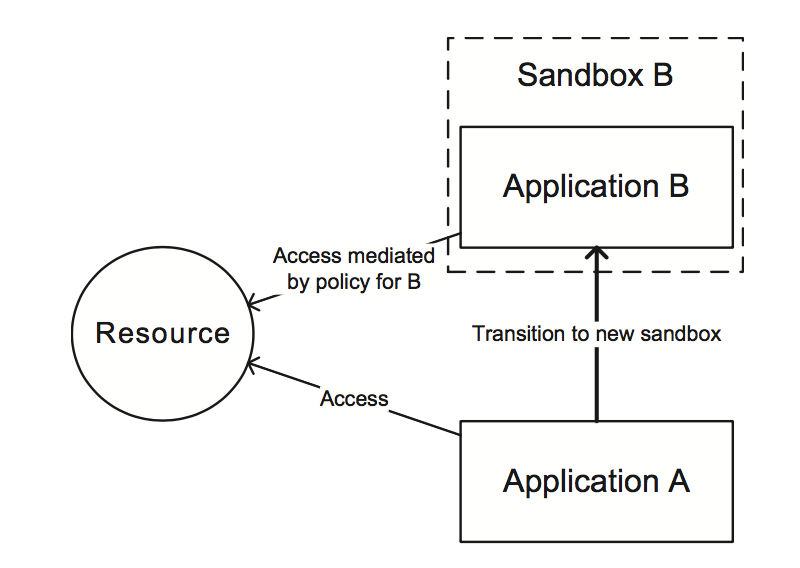
\includegraphics[width=0.4\linewidth]{imgs/type-2-sandbox.png}
}
\caption{沙箱分类}
\end{figure*}

沙箱技术大致可以被分为两类,其中第一类是基于隔离的沙箱,该类型的沙箱将应用的执行环境从操作系统中隔离出来,形成一个独立的执行环境。图 \ref{fig:t1sb} 展示了一个经典的基于隔离的沙箱模型。一个应用程序会在启动另一个应用程序之前先启动应用程序的沙箱,然后在沙箱内运行该应用程序,沙箱内的应用程序只能访问到沙箱内的资源。广为人知的虚拟机,容器,和传统意义上的沙箱都是这一类的沙箱模型。

第二类是基于规则的沙箱,该类型的沙箱并不是完全关注于对于应用程序的隔离上,而是用规则的方式控制每个应用的权限,基于规则的沙箱之间可以分享操作系统的逻辑资源。图 \ref{fig:t2sb} 展示了第二类的沙箱模型,不同于基于隔离的沙箱模型的地方在于,基于规则的沙箱模型并没有实现完全的资源隔离,而是对于每个应用,有不同的限制策略,通过强制应用限制策略来保证资源的访问权限受控 \cite{schreuders}。

由于篇幅限制,本文不能面面俱到地对各种沙箱技术都予以介绍,为了保证深度,本文选取第一类沙箱中的 Software-based Fault Isolation,以及第二类沙箱中的 System Call Interposition 和 Capabilities,来介绍沙箱技术的应用场景与实现,以及各自的优缺点,并在文末展开对各种技术的实现原理和潜在研究点的讨论。

\section{威胁模型}
\label{s:threat_model}

目前在互联网上,不受信任的应用的数量正在快速增长,让不受信任的应用程序能够更好地运行在系统中,是一件相当困难的事情。这些不受信用的应用程序可能隐藏有带有攻击意图的代码,它们获取操作系统高权限、读取文件系统中的敏感数据(比如密码、照片、文档等)、植入广告、导致系统崩溃等等。而攻击手段有很多,其中包括代码注入、Cross Site Scripting(CSS)、缓冲区溢出、Return-oriented programming(ROP) 等等 \cite{miwa}。

传统的操作系统并没有很好地解决这方面的问题,在隔离方面,仅仅依靠运行时的简单隔离是不够的。新的趋势使得操作系统应该在处理器,内存等硬件层面和进程,文件系统等软件层面进行更加细致的隔离和容错。这也是沙箱技术关注的焦点。沙箱技术有很多种,它们实现的方式也是不同的,但是其目的都是为了限制代码的运行,给予其隔离的运行环境。

// TODO:完善威胁模型

\section{Sandboxing 相关技术以及使用场景}
\label{s:implementation}

为了能够深入浅出地进行介绍,方便理解,本节将以一个现代的浏览器作为应用场景进行切入,在浏览器上,沙箱有着非常多的应用:

\begin{itemize}
\item
网页应用,现代的浏览器会在沙箱中运行你打开的网页代码。诸如 Javascript 之类的网页代码在浏览器的沙箱中只有有限的权限,它们并不能直接与文件系统等等进行交互,因此 Javascript 中的恶意代码的破坏性仅限于在沙箱内。
\item
浏览器插件,浏览器并不会直接将插件进程运行在操作系统上,而是会将其运行在一个沙箱进程中。比如 Adobe Flash 插件,就是如此。这样的隔离方式使得插件如同网页应用一样不能直接与操作系统进行交互,防止两者之间相互的攻击。
\item
各类下载内容的查看器,以 PDF 文件为例,浏览器下载的 PDF 文件会使用系统内的 PDF 阅读器打开,目前一些 PDF 阅读器正在使用沙箱技术来解析 PDF 文件,其中最有名的是 Adobe Reader。它运行在一个沙箱中,因此如果 PDF 文件中有恶意内容,也不会影响到操作系统。
\item
浏览器本身,浏览器是沙箱技术运用最广泛的桌面应用之一。浏览器不止将其请求的网页应用和插件等运行在容器中,浏览器本身也是运行在一个独立而隔离的沙箱中的。低权限的沙箱运行可以保证即使恶意内容破坏了网页应用所在的沙箱,也会被浏览器的沙箱所限制\footnote{http://www.howtogeek.com/169139/sandboxes-explained-how-theyre-already-protecting-you-and-how-to-sandbox-any-program/}。
\end{itemize}

本节将介绍 System Call Interposition(SCI)、Software-based Fault Isolation(SFI) 和 Capabilities 等技术在浏览器中的体现。System Call Interposition(SCI) 通过对系统调用的跟踪和限制,来使得应用不可以调用一些敏感的系统调用,或者不能将敏感的参数传入到系统调用中。Software-based Fault Isolation(SFI) 通过对指令的重写,使得应用运行时的故障不会往外传播,同时在一定程度上限制了代码的控制流。Capability Security Model(CSM)是一种区别于对服务提供者进行诸如Acccess Control List(ACL)的权限检查,而将权限检查绑定在被需要的实体上的一种设计理念\footnote{http://wiki.c2.com/?CapabilitySecurityModel}。这是三种完全不同的思路,它们的目的都是隔离代码的运行环境,构建出一个高度隔离的,低特权级的沙箱环境。

\subsection{System Call Interposition(SCI)}
\label{ss:sci}

在浏览器中,有很多互联网上的内容是需要下载,然后使用本地的查看器打开的。比如 PDF 文件等,需要通过 Adobe Reader 等专用软件打开。但是下载的内容有可能是隐藏有恶意代码的,但是本地的查看器并不一定将其视为不可信的内容,因此下载的内容在被相应的查看器打开时,恶意代码可能会被错误地执行了。对 System Call Interposition(以下称为 SCI)的研究,最开始的动机就是如何限制打开浏览器下载内容的助手应用,希望能够限制助手应用本身进行系统调用的权限。Janus\cite{goldberg}是 Goldberg 在 1996 年发表的论文,也是第一个成型的 SCI 系统实现,是这一领域奠基性的论文。随后有很多相关研究就此展开,研究者们继续完善 Janus,并且提出了新的解决思路。Ostia\cite{garfinkel}是 2004 年被提出的,它指出 Janus 存在很多缺点,而这些缺点的产生是因为架构问题,而不是 SCI 所固有的。因此它提出了一种新的架构,并且验证了他们的工作是比 Janus 的实现要高效而且可以解决 Janus 的缺点与问题。

\subsubsection{Janus}
\label{sss:janus}

// TODO

\subsubsection{Ostia}
\label{sss:ostia}

// TODO

\subsection{Software-based Fault Isolation(SFI)}
\label{ss:sfi}

浏览器是一个泛用性很强的应用,因此浏览器要求支持以插件的方式进行功能扩展。同时,为了提高浏览器中代码执行的性能,目前很多浏览器都在探索在浏览器中执行 Native 代码的方法。其中谷歌浏览器支持将 Native 代码运行在一个使用 Software-based Fault Isolation(以下称为 SFI) 的沙箱中。SFI 是在 1994 年在 Wahbe 的论文中第一次出现的\cite{wahbe1994efficient},SFI 通过修改程序二进制的方式,使得程序的二进制代码符合一些规则,来完成对于错误的隔离。在后来的论文中,谷歌结合了 SFI 和其他的一些沙箱技术,实现了一个面向 Native 代码运行环境的沙箱,这项技术一直到现在仍在被谷歌 Chrome 浏览器使用\cite{nacl}。

\subsubsection{Efficient Software-based Fault Isolation}
\label{sss:esfi}

// TODO

\subsubsection{Native Client}
\label{sss:nacl}

// TODO

\subsection{Capabilities}
\label{ss:capabilities}

// TODO: 加一段浏览器使用场景的引入

早在1988年,Normhardy就提出了confused deputies problem\cite{deputies}问题,并借此指出了capability的意义与价值。Confused deputies problem的场景可以大致描述为,一个程序需要在执行不同任务的时候,分别取得了不同的权限,这里的权限与前述的任务一一对应,但是一些恶意行为会混淆这里的权限与任务的对应,从而使得程序具有了执行不可预计的行为的权限,即其根本原因在于程序行为与其所拥有的权限之间的映射关系没能被很好的维护。但是在处理这个问题的时候,传统的基于ACL机制的解决方法往往会使得这个维护过程极其复杂,尤其当这里的映射关系的种类和数量变得繁多的时候,哪怕只是更新一个映射,其所带来的边际成本都会是递增的。同时,在这个问题上,"blame the user"(在这里,user是程序本身)是不合理的,而是应该是由OS来应对这个安全问题\footnote{http://wiki.c2.com/?ConfusedDeputyProblem}。Capability作为一种被认为是可行的解决方案,其核心思想是

// TODO: 核心思想 + 可靠(与ACL从效果上一致)

而Capability-based Security由于性能上的问题,大都被OS发行商所拒绝,很少出现在商业化的OS上。Capsicum\cite{capsicum}作为被纳入FreeBSD的一个基于capability的安全框架,是主要的一种系统级别的实现方式,并被Chromium作为其在FreeBSD下的安全基础\footnote{https://wiki.freebsd.org/Chromium}。下文将以此作为样例,展开阐述capability在系统级实现中的相关细节。

\subsubsection{设计思路}
\label{sss:design}

// TODO: 设计思路 + 涉及到的系统改动
//记得解释 principle of least privilege以及ambient authority

\subsubsection{应用调整}
\label{sss:adoption}

// TODO: 应用的相应调整 + 效果

而实际上,即使不在系统级别上实现capability-based security,依旧可以从编程的角度,进行capability-oriented programming\footnote{http://wiki.c2.com/?CapabilityOrientedProgramming}。

\section{Sandboxing 各种实现的分析与对比}
\label{s:evaluation}

\section{讨论与总结}
\label{s:tucao}


%% The Appendices part is started with the command \appendix;
%% appendix sections are then done as normal sections
%% \appendix

%% \section{}
%% \label{}

%% If you have bibdatabase file and want bibtex to generate the
%% bibitems, please use
%%
%%  \bibliographystyle{elsarticle-num} 
%%  \bibliography{<your bibdatabase>}

%% else use the following coding to input the bibitems directly in the
%% TeX file.

\clearpage

\section*{参考文献}

\bibliographystyle{elsarticle-num} 
\bibliography{myref}

\end{document}
\endinput
%%
%% End of file `elsarticle-template-num.tex'.
